\RequirePackage{atbegshi}
\documentclass[compress,aspectratio=169]{beamer}\usepackage[]{graphicx}\usepackage[dvipsnames]{xcolor}
% maxwidth is the original width if it is less than linewidth
% otherwise use linewidth (to make sure the graphics do not exceed the margin)
\makeatletter
\def\maxwidth{ %
  \ifdim\Gin@nat@width>\linewidth
    \linewidth
  \else
    \Gin@nat@width
  \fi
}
\makeatother

\definecolor{fgcolor}{rgb}{0.345, 0.345, 0.345}
\newcommand{\hlnum}[1]{\textcolor[rgb]{0.686,0.059,0.569}{#1}}%
\newcommand{\hlsng}[1]{\textcolor[rgb]{0.192,0.494,0.8}{#1}}%
\newcommand{\hlcom}[1]{\textcolor[rgb]{0.678,0.584,0.686}{\textit{#1}}}%
\newcommand{\hlopt}[1]{\textcolor[rgb]{0,0,0}{#1}}%
\newcommand{\hldef}[1]{\textcolor[rgb]{0.345,0.345,0.345}{#1}}%
\newcommand{\hlkwa}[1]{\textcolor[rgb]{0.161,0.373,0.58}{\textbf{#1}}}%
\newcommand{\hlkwb}[1]{\textcolor[rgb]{0.69,0.353,0.396}{#1}}%
\newcommand{\hlkwc}[1]{\textcolor[rgb]{0.333,0.667,0.333}{#1}}%
\newcommand{\hlkwd}[1]{\textcolor[rgb]{0.737,0.353,0.396}{\textbf{#1}}}%
\let\hlipl\hlkwb

\usepackage{framed}
\makeatletter
\newenvironment{kframe}{%
 \def\at@end@of@kframe{}%
 \ifinner\ifhmode%
  \def\at@end@of@kframe{\end{minipage}}%
  \begin{minipage}{\columnwidth}%
 \fi\fi%
 \def\FrameCommand##1{\hskip\@totalleftmargin \hskip-\fboxsep
 \colorbox{shadecolor}{##1}\hskip-\fboxsep
     % There is no \\@totalrightmargin, so:
     \hskip-\linewidth \hskip-\@totalleftmargin \hskip\columnwidth}%
 \MakeFramed {\advance\hsize-\width
   \@totalleftmargin\z@ \linewidth\hsize
   \@setminipage}}%
 {\par\unskip\endMakeFramed%
 \at@end@of@kframe}
\makeatother

\definecolor{shadecolor}{rgb}{.97, .97, .97}
\definecolor{messagecolor}{rgb}{0, 0, 0}
\definecolor{warningcolor}{rgb}{1, 0, 1}
\definecolor{errorcolor}{rgb}{1, 0, 0}
\newenvironment{knitrout}{}{} % an empty environment to be redefined in TeX

\usepackage{alltt}

% % % % % % % % % % % % % % %
%             MY PACKAGES 
% % % % % % % % % % % % % % %
\usepackage{graphicx}
\usepackage{dcolumn}
\usepackage[export]{adjustbox}
\usepackage[dvipsnames]{xcolor}
\usepackage{amssymb,amsmath}
\usepackage{threeparttable}

\usepackage{pgfplots}
\pgfplotsset{compat=1.11}
\usepgfplotslibrary{fillbetween}

\usepackage{rotating}
\usepackage{import}
\usepackage{array}
\usepackage{tabularx}
\usepackage{float}
\usepackage{pifont}
\usepackage{hyperref}
\usepackage{multirow}

\usepackage{tikz}
\usetikzlibrary{arrows,decorations.pathreplacing,positioning,shapes.geometric}


\usepackage{listings}
\usepackage{color}
\definecolor{dkgreen}{rgb}{0,0.6,0}
\definecolor{gray}{rgb}{0.5,0.5,0.5}
\definecolor{mauve}{rgb}{0.58,0,0.82}
\lstset{
  language=R,
  basicstyle=\TINY,
  numbers=left,
  numberstyle=\tiny\color{gray},
  stepnumber=1,
  numbersep=5pt,
  backgroundcolor=\color{white},
  showspaces=false,
  showstringspaces=false,
  showtabs=false,
  frame=single,
  rulecolor=\color{black},
  tabsize=1,
  captionpos=b,
  breaklines=true,
  breakatwhitespace=false,
  title=\lstname,
  keywordstyle=\color{blue},
  commentstyle=\color{dkgreen},
  stringstyle=\color{mauve},
  escapeinside={\%*}{*)},
  morekeywords={*,...}
}

% % % % % % % % % % % % % % %
%           PACKAGE CUSTOMIZATION
% % % % % % % % % % % % % % %

\usepackage[math]{iwona}
\usetheme{Singapore}
\usecolortheme{rose}
\makeatletter
\beamer@theme@subsectiontrue
\makeatother

% navigation dots behavior
\makeatletter
\def\slideentry#1#2#3#4#5#6{%
  \ifnum#6=\c@part\ifnum#2>0\ifnum#3>0%
    \ifbeamer@compress%
      \advance\beamer@xpos by1\relax%
    \else%
      \beamer@xpos=#3\relax%
      \beamer@ypos=#2\relax%
    \fi%
  \hbox to 0pt{%
    \beamer@tempdim=-\beamer@vboxoffset%
    \advance\beamer@tempdim by-\beamer@boxsize%
    \multiply\beamer@tempdim by\beamer@ypos%
    \advance\beamer@tempdim by -.05cm%
    \raise\beamer@tempdim\hbox{%
      \beamer@tempdim=\beamer@boxsize%
      \multiply\beamer@tempdim by\beamer@xpos%
      \advance\beamer@tempdim by -\beamer@boxsize%
      \advance\beamer@tempdim by 1pt%
      \kern\beamer@tempdim
      \global\beamer@section@min@dim\beamer@tempdim
      \hbox{\beamer@link(#4){%
          \usebeamerfont{mini frame}%
          \ifnum\c@section>#1%
            \usebeamercolor{mini frame}%
            \usebeamertemplate{mini frame in other subsection}%
          \else%
            \ifnum\c@section=#1%
              \ifnum\c@subsection>#2%
                \usebeamercolor[fg]{mini frame}%
                \usebeamertemplate{mini frame}%
              \else%
                \ifnum\c@subsection=#2%
                  \usebeamercolor[fg]{mini frame}%
                  \ifnum\c@subsectionslide<#3%
                    \usebeamertemplate{mini frame in current subsection}%
                  \else%
                    \usebeamertemplate{mini frame}%
                  \fi%
                \else%
                  \usebeamercolor{mini frame}%
                  \usebeamertemplate{mini frame in other subsection}%
                \fi%
              \fi%
            \else%
              \usebeamercolor{mini frame}%
              \usebeamertemplate{mini frame in other subsection}%
            \fi%
          \fi%
        }}}\hskip-10cm plus 1fil%
  }\fi\fi%
  \else%
  \fakeslideentry{#1}{#2}{#3}{#4}{#5}{#6}%
  \fi\ignorespaces
}
\makeatother

\beamertemplatenavigationsymbolsempty
\makeatletter
\setbeamertemplate{footline}{
\leavevmode%
\hbox{%
\begin{beamercolorbox}[wd=1\paperwidth,ht=2.25ex,dp=2ex,center]{title in head/foot}%
\usebeamerfont{title in head/foot}\insertshorttitle
\end{beamercolorbox}%
\begin{beamercolorbox}[wd=1\paperwidth,ht=2.25ex,dp=2ex,center]{date in head/foot}%
\end{beamercolorbox}}%
}
\makeatother

\makeatletter
\let\beamer@writeslidentry@miniframeson=\beamer@writeslidentry
\def\beamer@writeslidentry@miniframesoff{%
  \expandafter\beamer@ifempty\expandafter{\beamer@framestartpage}{}%
  {%
    \clearpage\beamer@notesactions%
  }
}
\newcommand*{\miniframeson}{\let\beamer@writeslidentry=\beamer@writeslidentry@miniframeson}
\newcommand*{\miniframesoff}{\let\beamer@writeslidentry=\beamer@writeslidentry@miniframesoff}
\makeatother

\newcommand<>{\fullsizegraphic}[1]{
  \begin{textblock*}{0cm}(-1cm,-3.78cm)
  \includegraphics[width=\paperwidth]{#1}
  \end{textblock*}
}

\hypersetup{colorlinks,urlcolor=[rgb]{0.01,0.28,1.0},linkcolor=[rgb]{0.01,0.28,1.0}}

% % % % % % % % % % % % % % %
%           DOCUMENT ID
% % % % % % % % % % % % % % %

\title{\input{title.txt}\unskip}
\author[shortname]{Hector Bahamonde \inst{1} \and Andrea Canales \inst{2}}
\institute[shortinst]{\inst{1} University of Turku, Finland \and \inst{2} O$'$Higgins University, Chile}
\date{Dec 11th 2026}
\IfFileExists{upquote.sty}{\usepackage{upquote}}{}
\begin{document}





%====================
% TITLE SLIDE
%====================

\begin{frame}
\titlepage
\end{frame}

%====================
% INTRODUCTION
%====================

\section{Introduction}
\subsection{Motivation}

\miniframesoff
\begin{frame}[c]{Today we're gonna talk about sequencing}

\begin{itemize}
  \item \textbf{Welfare state and unions:} Do we get different welfare states when \emph{unions first mobilize} before benefits expand, versus when \emph{governments move first} potentially avoiding workers' needs?

  \item \textbf{Intergenerational inequality:} What happens to class reproduction when \emph{parents must invest first} (education, housing, debt) and the state steps in later, versus systems where \emph{the state introduces first} universal support?

  \item {\color{blue}Sequencing might really change social outcomes, making losers and winners depending on who plays first}.

  %\item \textbf{Access to medicine and care:} Who lives longer when \emph{patients must ask, apply, and fight} for treatment first, versus systems where \emph{the welfare state moves first} and automatically enrolls, screens, and follows up?

  %\item \textbf{Fertility and family formation:} Would people have more children if \emph{childcare, housing, and income supports arrive before the first baby}, instead of after? In low-natality societies, is the problem \emph{resources}, or the \emph{order in which they arrive}?
\end{itemize}
\end{frame}


\miniframeson
\usetikzlibrary{arrows,decorations.pathreplacing,positioning,calc}

\begin{frame}[c]{How Sequencing Changes the Frame}
\begin{columns}[T,totalwidth=\textwidth]

  %%%%% LEFT COLUMN %%%%%
  \begin{column}{0.55\textwidth}
    \begin{itemize}
      \item[] \underline{\textbf{Notice how the sequence flips the frame}}:
      \smallskip
      \item Friend (unexpectedly) \textbf{offers} you 50€: you might see them as (unexpected) \textbf{gains}.
      \item You sell the same good but \textbf{demand} 80€: now you fear \textbf{losses}.
\end{itemize}

    \bigskip

    \begin{itemize}
      \item[\checkmark] {\color{blue}My talk will be about sequencing in clientelism}.
    \end{itemize}
  \end{column}

  %%%%% RIGHT COLUMN %%%%%
  \begin{column}{0.45\textwidth}
    \centering
    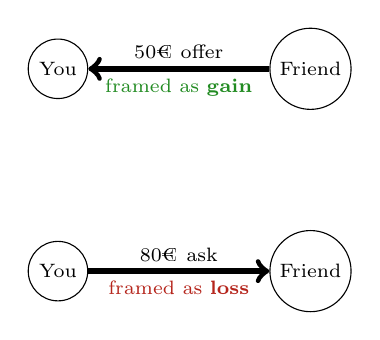
\begin{tikzpicture}[node distance=1.4cm]
      \scriptsize

      % Top: friend offers 50€ → framed as gain
      \node[circle,draw,minimum size=0.7cm] (you1) {You};
      \node[circle,draw,minimum size=0.7cm,right=2.3cm of you1] (fr1) {Friend};

      \draw[->,line width=2pt]
        (fr1) -- node[above]{50€ offer}
                 node[below,text=ForestGreen]{framed as \textbf{gain}}
        (you1);

      % Bottom: you demand 80€ → framed as loss
      \node[circle,draw,minimum size=0.7cm,below=1.8cm of you1] (you2) {You};
      \node[circle,draw,minimum size=0.7cm,right=2.3cm of you2] (fr2) {Friend};

      \draw[->,line width=2pt]
        (you2) -- node[above]{80€ ask}
                 node[below,text=BrickRed]{framed as \textbf{loss}}
        (fr2);

    \end{tikzpicture}

    \vspace{0.3cm}
    {\bf Who moves first can reshape the deal}
    %\begin{exampleblock}{{\scriptsize Who moves first can reshape the deal.}}
    %  {\scriptsize Move second, and become a \textbf{price taker}.}
    %\end{exampleblock}

  \end{column}

\end{columns}
\end{frame}








\subsection{Definition and geographical relevance}

\miniframeson
\begin{frame}[c]{}

{\bf Clientelism}: distribution of private rewards to individuals during elections in exchange for electoral support {\scriptsize{\color{gray}(Nichter, 2014)}}.

\vspace{0.5cm}

\uncover<2->{\large {\color{blue}Essentially, cash for your vote}.}

\vspace{0.8cm}

\centering
\includegraphics[scale=0.3]{/Users/hectorbahamonde/research/Economic_Experiment_Vote_Selling/Resources_Presentation/vote_buying.jpg}

\end{frame}


\miniframesoff
\begin{frame}[c]{}

  \includegraphics[scale=0.27, center]{/Users/hectorbahamonde/research/Exp_Vote_Selling/clientelism_vdem_index_2024.png}


\end{frame}


\miniframeson
\subsection{Gaps in the literature}

\begin{frame}[c]{Sequencing has been Overlooked}
\begin{itemize}
  

  \item {\bf Ethnographers}: voters, neighborhood leaders, and brokers (potential {\bf sellers}) often {\bf begin} exchanges.


  \item {\bf Quantitative}: usually show clientelism as \textbf{party-initiated demand} for votes.\pause

 

  \item[\checkmark] {\color{blue} Sequencing has been overlooked in the quantitative literature}:
  \begin{itemize}
    \item Heavily focused on {\bf vote buying}.
    \item Very few studies {\bf vote selling}.
    %\item Almost none treat buyers and sellers symmetrically.
  \end{itemize}
  \item[\checkmark] {\color{blue} We argue: to understand clientelism, put \textbf{voters as strategic sellers} (just like vote-buying parties)}.
\end{itemize}
\end{frame}


\miniframesoff
\begin{frame}[c]{Sequencing has been Overlooked}
\centering
\includegraphics[width=0.75\textwidth]{/Users/hectorbahamonde/research/Exp_Vote_Selling/histogram_meta_plot_wide.pdf}
\vspace{0.2cm}

{\tiny Annual frequency of Web of Science publications whose abstracts include the terms ``vote buying'' and ``vote selling.''}
\end{frame}



\subsection{Our contribution}

\miniframeson
\begin{frame}[c]{Our Paper and Today's Talk}
\begin{itemize}
  \item {\bf Conceptual move}: integrate {\color{red}vote buying} \emph{and} {\color{blue}vote selling} in the same framework.\pause
  \item {\bf Theory}: formalize a spatial model with one voter and two parties.

    \begin{enumerate}
            \item {\color{red}Parties moves first}.
            \item {\color{blue}Voters moves first}.

    \end{enumerate}\pause


  
  \item {\bf Experiment}: based on the spatial model, we designed a lab experiment.\pause

  
  \item {\bf Findings}:
  \begin{itemize}
    \item[\checkmark] {\color{red}When parties move first}: transfers concentrate on \textbf{party supporters}.
    \item[\checkmark] {\color{blue}When voters move first}: they \textbf{demand higher prices} from winning parties that are ideologically far away.
    \item[\checkmark] Voters earn \textbf{higher payoffs} when parties initiate the exchange.
  \end{itemize}
\end{itemize}
\end{frame}

%====================
% THEORY
%====================

\section{Theory}

\subsection{Formalization}


%====================
% THEORY (clean, non-overlay version)
%====================

\miniframeson
\begin{frame}[c]{A Uni-dimensional Spatial Theory of Voting}
\begin{columns}[T,totalwidth=\textwidth]

% LEFT: intuition
\begin{column}{0.55\textwidth}
\begin{itemize}[<+->]
  \item Politics lives on a simple \textbf{left--right space}. {\scriptsize \color{gray}\(\gamma \in \Gamma = \{1,\dots,100\}\)}
  \item Two parties positioned on that space.\\
  {\scriptsize \color{gray}\(i \in \{A,B\}\), at \(\gamma_A,\gamma_B\)}
  \item Parties care about \textbf{winning the election}.\\
  {\scriptsize \color{gray} \(W_i\); electoral stake \(R_i = \pi W_i\)}
  \item Voters care about \textbf{ideological proximity} and {\bf not losing the election}.\\
  {\scriptsize \color{gray}ideal point \(x_j\), utility \(u_j(\gamma_i)\)}
\end{itemize}

\end{column}

% RIGHT: spatial intuition
\begin{column}{0.45\textwidth}
\centering
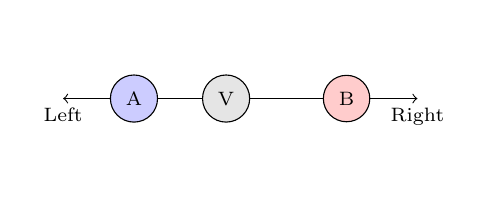
\begin{tikzpicture}[scale=0.9,baseline=(axis)]

  % --- FIXED BOUNDING BOX (same in all frames) ---
  \path (-0.5,-1.0) (5.5,1.0);

  % axis anchor (used for baseline)
  \coordinate (axis) at (2.5,0);

  % axis
  \draw[<->] (0,0) -- (5,0);
  \node[below] at (0,0) {\scriptsize Left};
  \node[below] at (5,0) {\scriptsize Right};

  % parties
  \onslide<2->{
    \node[circle,draw,fill=blue!20] at (1,0) {\scriptsize A};
    \node[circle,draw,fill=red!20]  at (4,0) {\scriptsize B};
  }

  % voter (circle to avoid 'diamond' errors)
  \onslide<4->{
    \node[circle,draw,fill=gray!20] at (2.3,0) {\scriptsize V};
  }

\end{tikzpicture}

\onslide<5->{
\begin{block}{Key idea}
{\scriptsize Voters face a \textbf{tradeoff between ideological utility} {\tiny \color{gray}\(u_j(\gamma_i)\)} \textbf{and electoral risk} {\tiny \color{gray}\(R_i=\pi W_i\)}.}
\end{block}
}


\end{column}

\end{columns}
\end{frame}



\miniframesoff
\begin{frame}[c]{A Uni-dimensional Spatial Theory of Voting}
\begin{columns}[T,totalwidth=\textwidth]

% LEFT
\begin{column}{0.55\textwidth}
\begin{itemize}[<+->]
  \item Ideological advantage {\scriptsize \color{gray}\(\Delta\)}
  \item The voter gets more utility {\scriptsize \color{gray}\(\Delta\)} from the closer party {\scriptsize \color{gray}\(u_j(\gamma_i)\)}
\end{itemize}

\medskip
\onslide<3->{
\begin{block}{Implication}
\(\Delta\) represents the minimum compensation (minimal transfer) the voter needs to switch sides.
\end{block}
}
\end{column}

% RIGHT
\begin{column}{0.45\textwidth}
\centering
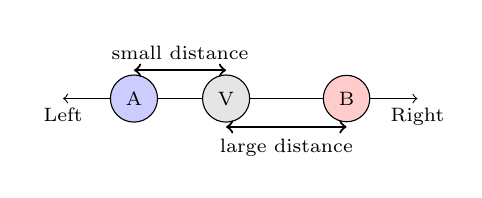
\begin{tikzpicture}[scale=0.9,baseline=(axis)]

  % --- FIXED BOUNDING BOX (same in all frames) ---
  \path (-0.5,-1.0) (5.5,1.0);

  % axis anchor
  \coordinate (axis) at (2.5,0);

  % axis
  \draw[<->] (0,0) -- (5,0);
  \node[below] at (0,0) {\scriptsize Left};
  \node[below] at (5,0) {\scriptsize Right};

  % parties
  \onslide<1->{
    \node[circle,draw,fill=blue!20] at (1,0) {\scriptsize A};
    \node[circle,draw,fill=red!20]  at (4,0) {\scriptsize B};
  }

  % voter
  \onslide<2->{
    \node[circle,draw,fill=gray!20] at (2.3,0) {\scriptsize V};
  }

  % distances
  \onslide<3->{
    \draw[<->,thick] (1,0.4) -- (2.3,0.4);
    \node at (1.65,0.65) {\scriptsize small distance};

    \draw[<->,thick] (2.3,-0.4) -- (4,-0.4);
    \node at (3.15,-0.7) {\scriptsize large distance};
  }

\end{tikzpicture}
\end{column}

\end{columns}
\end{frame}




\miniframesoff
\begin{frame}[c]{A Uni-dimensional Spatial Theory of Voting}
\begin{columns}[T,totalwidth=\textwidth]

% LEFT
\begin{column}{0.55\textwidth}
\begin{itemize}[<+->]
  \item Sometimes, both parties run in tight races. {\scriptsize \color{gray}High pivotality \(\pi\)}
  \item That voter is \textbf{pivotal} {\scriptsize \color{gray}(with probability \(\pi>0\))}.
\end{itemize}

\medskip
\onslide<3->{
\begin{block}{Implication}
  \(R_i\) represents how worthy winning is, determining the voter's price.
\end{block}
}
\end{column}

% RIGHT
\begin{column}{0.45\textwidth}
\centering
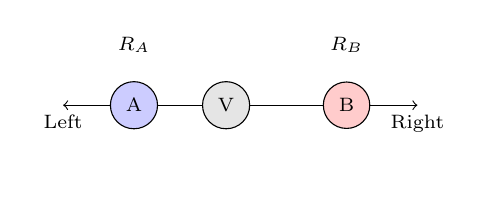
\begin{tikzpicture}[scale=0.9,baseline=(axis)]

  % --- FIXED BOUNDING BOX (same in all frames) ---
  \path (-0.5,-1.0) (5.5,1.0);

  % axis anchor
  \coordinate (axis) at (2.5,0);

  % axis
  \draw[<->] (0,0) -- (5,0);
  \node[below] at (0,0) {\scriptsize Left};
  \node[below] at (5,0) {\scriptsize Right};

  % parties
  \onslide<1->{
    \node[circle,draw,fill=blue!20] at (1,0) {\scriptsize A};
    \node[circle,draw,fill=red!20]  at (4,0) {\scriptsize B};
  }

  % voter
  \onslide<2->{
    \node[circle,draw,fill=gray!20] at (2.3,0) {\scriptsize V};
  }

  % stakes
  \onslide<3->{
    \node[above] at (1,0.6) {\scriptsize $R_A$};
    \node[above] at (4,0.6) {\scriptsize $R_B$};
  }

\end{tikzpicture}
\end{column}

\end{columns}
\end{frame}


\miniframesoff
\begin{frame}[c]{A Uni-dimensional Spatial Theory of Voting}
\begin{columns}[T,totalwidth=\textwidth]

% LEFT
\begin{column}{0.55\textwidth}
\begin{itemize}[<+->]
  \item {\color{blue}When parties begin}, they make offers {\scriptsize \color{gray}\(s_A, s_B\)}.
  \item The voter compares ideology \(\,+\) offers and chooses a party\\
  {\scriptsize \color{gray}\(i \in \{A,B\}\) to maximize \(U_j(i,s_i)\)}
\end{itemize}

\medskip
\onslide<3->{
\begin{block}{Key result}
It is cheapest to buy the vote from the \textbf{core voter} {\scriptsize \color{gray}(\(i^\ast\), with advantage \(\Delta\))}.
\end{block}
}
\end{column}

% RIGHT
\begin{column}{0.45\textwidth}
\centering
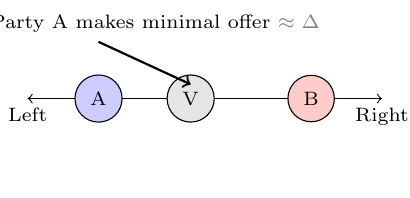
\begin{tikzpicture}[scale=0.9,baseline=(axis.base)]
  % FIXED bounding box
  \path[use as bounding box] (0,-1.0) rectangle (5,1.0);

  % axis
  \coordinate (axis) at (2.5,0);
  \draw[<->] (0,0) -- (5,0);
  \node[below] at (0,0) {\scriptsize Left};
  \node[below] at (5,0) {\scriptsize Right};

  % parties
  \node[circle,draw,fill=blue!20] at (1,0) {\scriptsize A};
  \node[circle,draw,fill=red!20]  at (4,0) {\scriptsize B};

  % voter
  \node[circle,draw,fill=gray!20] at (2.3,0) {\scriptsize V};

  % offer from core party (assume A is core)
  \onslide<2->{
    \draw[->,thick] (1,0.8) -- (2.3,0.2);
    \node[above] at (1.8,0.8) {\scriptsize Party A makes minimal offer {\scriptsize \color{gray}\(\approx \Delta\)}};
  }

\end{tikzpicture}
\end{column}

\end{columns}
\end{frame}




\miniframesoff
\begin{frame}[t]{A Uni-dimensional Spatial Theory of Voting}
\begin{columns}[T,totalwidth=\textwidth]

% LEFT
\begin{column}{0.55\textwidth}
\begin{itemize}[<+->]
  \item {\color{blue}When the voter begins}, they send offers {\scriptsize \color{gray}\(a_A, a_B\)}.
  \item Parties accept or reject offers\\ {\scriptsize \color{gray}\(R_i\); accepting when \(a_i \le R_i\)}
\end{itemize}

\medskip
\onslide<3->{
\begin{block}{Implication}
Voters ask more from parties with \textbf{more to lose} {\scriptsize\color{gray}(big \(R_i\))}.
\end{block}
}
\end{column}

% RIGHT
\begin{column}{0.45\textwidth}
\centering
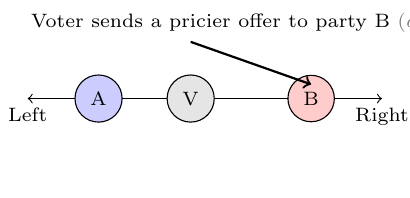
\begin{tikzpicture}[scale=0.9,baseline=(axis.base)]
  % FIXED bounding box
  \path[use as bounding box] (0,-1.0) rectangle (5,1.0);

  % axis
  \coordinate (axis) at (2.5,0);
  \draw[<->] (0,0) -- (5,0);
  \node[below] at (0,0) {\scriptsize Left};
  \node[below] at (5,0) {\scriptsize Right};

  % parties: let B be electorally stronger
  \node[circle,draw,fill=blue!20] at (1,0) {\scriptsize A};
  \node[circle,draw,fill=red!20]  at (4,0) {\scriptsize B};

  % voter
  \node[circle,draw,fill=gray!20] at (2.3,0) {\scriptsize V};

  % requests
  \onslide<3->{
    \draw[->,thick] (2.3,0.8) -- (4,0.2);
    \node[above] at (3.4,0.8) {\scriptsize Voter sends a pricier offer to party B {\scriptsize\color{gray}(\(a_B \approx R_B\))}};
  }

\end{tikzpicture}
\end{column}

\end{columns}
\end{frame}





\subsection{Hypotheses}


\miniframeson
\begin{frame}[c]{Formally Derived Hypotheses}
\begin{itemize}
  \item \textbf{H1 (Core Targeting Under Party Initiative):}
  \begin{itemize}
    \item When parties initiate, transfers concentrate on ideologically proximate voters; parties mainly buy from their followers.
  \end{itemize}
  \item \textbf{H2 (Selling to the Opponent Winning Party):}
  \begin{itemize}
    \item When voters initiate, they demand higher prices from electorally strong but ideologically distant parties.
  \end{itemize}
  \item \textbf{H3 (Higher Voter Payoffs Under Party Initiative):}
  \begin{itemize}
    \item Because parties overspend under electoral risk, voters earn higher expected payoffs in VB than in VS.
  \end{itemize}
\end{itemize}
\end{frame}

%====================
% EXPERIMENT
%====================

\section{Experimental design}

\subsection{Setup and roles}


\miniframeson
\begin{frame}[c]{Laboratory implementation}
\begin{itemize}
  \item \textbf{Subjects and implementation}
  \begin{itemize}
    \item Following the formal model, we designed a lab experiment in \texttt{oTree}.
    \item Recruited 102 adult participants.
    \item Payed them according to the quality of their decisions.
  \end{itemize}\pause
  
  \item \textbf{Roles}
  \begin{itemize}
    \item Each game: three (real) players (Party A, Party B, Voter).
    \item Each subject played the game three times (n=306).
    \item Every time we executed a new randomization block. 
  \end{itemize}\pause

  \item \textbf{What was randomized every time}
  \begin{itemize}
    \item Role (party, voter).
    \item Voter's ideological payoffs if {\bf A} or {\bf B} wins.
    \item Party budgets (to buy votes).
    \item If the voter is pivotal.
  \end{itemize}
\end{itemize}
\end{frame}


\subsection{Randomization}


\miniframeson
\begin{frame}[c]{Experimental Flow}
\centering
\includegraphics[width=\textwidth]{/Users/hectorbahamonde/research/Exp_Vote_Selling/experimental_flow.pdf}

\vspace{0.2cm}
{\small Two institutional variants in an otherwise identical strategic environment.}
\end{frame}

%====================
% EMPIRICAL RESULTS
%====================

\section{Empirical results}
\subsection{Dependent Variable}


\miniframeson
\begin{frame}[c]{The Dependent Variable: Vote-buying and vote-selling prices}
\begin{columns}[T,totalwidth=\textwidth]

% LEFT COLUMN: HISTOGRAMS
\begin{column}{0.6\textwidth}
\centering
\includegraphics[width=\textwidth]{/Users/hectorbahamonde/research/Exp_Vote_Selling/depvarplot.pdf}

%\vspace{0.1cm}
%{\scriptsize Distributions of vote-buying offers (left) and vote-selling requests (right), as a share of party budgets.}
\end{column}

% RIGHT COLUMN: INTERPRETATION
\begin{column}{0.4\textwidth}
\begin{itemize}
  \item The two histograms describe \textbf{very different worlds}:
  \begin{itemize}
    \item When \textbf{parties move first}.
    \item When \textbf{voters move first}.
  \end{itemize}

  \medskip

  \item \textbf{What explains the differences of these two games?}
\end{itemize}
\end{column}

\end{columns}
\end{frame}



\subsection{Modeling Vote Buying}


\miniframeson
\begin{frame}[c]{Modeling vote-buying offers}

\begin{itemize}
  \item {\bf What explains the variance of the vote-buying offers?} Estimate OLS:
\end{itemize}

\[
\text{Offer}_{di}
=
\gamma_0
+ \gamma_1 \only<2>{\textcolor{red}{\text{Ideology}_{di}}}\only<1,3,4>{\text{Ideology}_{di}}
+ \gamma_2 \only<3>{\textcolor{red}{\text{VoteShare}_{di}}}\only<1,2,4>{\text{VoteShare}_{di}}
+ \gamma_3 \only<4>{\textcolor{red}{\text{Pivotal}_d}}\only<1,2,3>{\text{Pivotal}_d}
+ u_{di}
\]

\begin{itemize}
  \item Also a logit model for the probability of making \emph{any} offer.
  \item  Standard errors clustered at the party level.
\end{itemize}

\end{frame}



\subsection{Results: Vote Buying}

\miniframeson
\begin{frame}[c]{Results: Vote-Buying Offers and Core Targeting}

\begin{columns}[c]

  % LEFT COLUMN: FIGURES (fixed height!)
  \column{0.55\textwidth}
  \centering

  \begin{overlayarea}{\textwidth}{5cm}

    \only<1>{
      \includegraphics[width=0.8\textwidth]{/Users/hectorbahamonde/research/Exp_Vote_Selling/H1_ideo_distance_plot.pdf}
    }

    \only<2>{
      \includegraphics[width=0.8\textwidth]{/Users/hectorbahamonde/research/Exp_Vote_Selling/H1_ols_presentation.pdf}
    }

    \only<3>{
      \includegraphics[width=\textwidth]{/Users/hectorbahamonde/research/Exp_Vote_Selling/H1_combined.pdf}
    }

  \end{overlayarea}

  % RIGHT COLUMN: INTERPRETATION (already fixed)
  \column{0.45\textwidth}

  \begin{overlayarea}{\textwidth}{4cm}
    \begin{itemize}
      \item<1-> As ideological distance increases, parties are \textbf{less likely} to make any offer at all.
      \item<2-> If they offer, parties pay \textbf{larger} transfers to more distant voters.
      \item<3-> So: parties target followers cheaply (right), but pay a premium to buy distant votes (left).
    \end{itemize}
  \end{overlayarea}

\end{columns}

\end{frame}






\subsection{Modeling Vote Selling}


\miniframeson
\begin{frame}[c]{Modeling vote-selling prices}

\begin{itemize}
  \item {\bf What explains how voters price their vote?} Estimate OLS:
\end{itemize}

\[
Y_{di}
=
\beta_0
+ \beta_1 \alert<2>{\text{Ideology}_{di}}
+ \beta_2 \alert<3>{\text{VoteShare}_{di}}
+ \beta_3 \alert<4>{\text{Ideology}_{di} \times \text{VoteShare}_{di}}
+ \beta_4 \alert<5>{\text{Pivotal}_d}
+ \varepsilon_{di}
\]

\begin{itemize}
  \item Dependent variable: requested price as \% of party budget,
  \[
    Y_{di} = \frac{a_{di}}{B_{di}} \times 100.
  \]
  \item Standard errors clustered at the voter level.
\end{itemize}

\end{frame}



\subsection{Results: Vote Selling}

\miniframeson
\begin{frame}[c]{Requested Prices by Ideology and Electoral Strength}

\begin{columns}[c]

  % LEFT COLUMN: FIGURE
  \column{0.5\textwidth}
  \centering
  \includegraphics[width=0.9\textwidth]{/Users/hectorbahamonde/research/Exp_Vote_Selling/m1plot.pdf}

  % RIGHT COLUMN: INTERPRETATION
  \column{0.5\textwidth}

  \begin{itemize}
    \item Voters ask for expensive transfers:
    \begin{itemize}
      \item When the {\bf weak} party is ideologically close but likely to lose (insurance against losses).
      \item When the party is {\bf strong} and distant (voters exploit electorally strong parties' higher electoral stakes $R_i$.)
    \end{itemize}
  \end{itemize}

\end{columns}

\end{frame}
 




\subsection{Timing: Institutional Differences}


\miniframeson
\begin{frame}[c]{Payoffs by Role and Institutional Variant}

\begin{columns}[c]

  % LEFT COLUMN: FIGURE
  \column{0.55\textwidth}
  \centering
  \includegraphics[width=0.9\textwidth]{/Users/hectorbahamonde/research/Exp_Vote_Selling/payoffs_plot.pdf}

  %\vspace{0.2cm}
  %{\footnotesize Mean payoffs for voters and parties under party-initiated vote buying (VB) and voter-initiated vote selling (VS). Error bars show non-parametric 90\% confidence intervals.}

  % RIGHT COLUMN: INTERPRETATION
  \column{0.45\textwidth}

  \begin{itemize}
    \item Party payoffs are similar across vote buying and vote selling.
    \item Voters earn \textbf{higher average payoffs} when parties begin the exchange.
    %\item In VB, parties overspend relative to the minimal compensating transfer ({\scriptsize$\Delta$}) under electoral risk.
    %\item In VS, very high requested prices are often rejected, leaving some voters with only ideological payoffs.
  \end{itemize}

\end{columns}

\end{frame}

%====================
% DISCUSSION
%====================

\section{Discussion}

\subsection{What we learned}


\miniframeson
\begin{frame}[c]{Main takeaways}
\begin{itemize}
  \item {\bf Conceptual move}: integrated {\color{red}vote buying} \emph{and} {\color{blue}vote selling} in the same framework.
  \item {\bf Theory}: formalized a spatial model with one voter and two parties.

    \begin{enumerate}
            \item {\color{red}Parties moved first}.
            \item {\color{blue}Voters moved first}.

    \end{enumerate}


  
  \item {\bf Experiment}: based on the formal model, we designed a lab econ experiment.

  
  \item {\bf Findings}:
  \begin{itemize}
    \item[\checkmark] {\color{red}When parties move first}: transfers concentrate on \textbf{party supporters}.
    \item[\checkmark] {\color{blue}When voters move first}: they \textbf{demand higher prices} from winning parties that are ideologically far away.
    \item[\checkmark] Voters earn \textbf{higher average payoffs} when parties initiate the exchange.
  \end{itemize}
\end{itemize}
\end{frame}



%====================
% END
%====================

\miniframesoff
\begin{frame}[c]{Thank you}
\begin{center}
\vspace{-0.5cm}
\includegraphics[scale=0.05]{/Users/hectorbahamonde/research/Economic_Experiment_Vote_Selling/Resources_Presentation/qr-code.pdf}
\end{center}
\begin{itemize}
  \item Paper and abstract: {\color{blue}www.HectorBahamonde.com}
  \item Feedback very welcome.
\end{itemize}
\end{frame}

\end{document}
